\documentclass[11pt]{beamer}
\usetheme{Warsaw}
\usepackage[utf8]{inputenc}
\usepackage{amsmath}
\usepackage{amsfonts}
\usepackage{amssymb}
\usepackage{graphicx}
\usepackage{pgfplotstable}
\usepackage{filecontents} %%%%
\author{Marco Stumper und Alexander Walter}
\title{Molecular Dynamics Simulation}
%\setbeamercovered{transparent} 
\setbeamertemplate{footline}[frame number] 
%\logo{
\includegraphics[height=1.5cm]{UHH.eps}}
\institute{Universität Hamburg} 
\date{\today} %vorraussichtlich 31.1.2014 

\titlegraphic{
    \vspace{0.9cm}
    \hspace*{2.3cm}
    \begin{minipage}{0.6\textwidth}
        
\includegraphics[height=1.5cm]{img/UHH.eps}
    \end{minipage}}
    
\subject{Molecular Dynamics Simulation} 

\begin{document}

\begin{frame}[plain]
  \titlepage
\end{frame}

\begin{frame}
  \begin{minipage}{0.50\textwidth}
	\frametitle{Molecular Dynamics}
	\tableofcontents
  \end{minipage}
  \begin{minipage}{0.45\textwidth}
  \hspace*{-1.3cm}
  \end{minipage}
\end{frame}


\section{Molecular Dynamics}

\subsection{Simulation}

\begin{frame}
  \frametitle{Erklärung}
  \vspace*{-0.3cm}
  \begin{block}{Grundlegendes}
    \begin{itemize}
      \item Es befinden sich N Partikel in einer 3D Box mit Seitenlängen L
      \item Dichte ${RHO = N/L^3}$
      \end{itemize}
  \end{block}
  \pause
  \begin{block}{Initialisierung}
    \begin{itemize}
      \item Die Partikel werden an zufälligen Orten platziert (Optional in einem Kasten)
      \item Die Box hat periodic boundary conditions %TODO
    \end{itemize}
  \end{block}
  \pause
  \begin{block}{Simulation}
    \begin{itemize}
      \item Ein Simulationsschritt wird mit Hilfe von 2 Arrays berechnet
      \item Wir verwenden das Lennard-Jones Potential
    \end{itemize}
  \end{block}
\end{frame}

\subsection{Potential}

\begin{frame}
  \frametitle{Lennard-Jones-Potential}
   \vspace{-0.2cm}
    \hspace*{+0.25cm}
    
\includegraphics[width=0.93\textwidth]{img/LennardJonesPotential.png}
\end{frame}

\begin{frame}
  \frametitle{Lennard-Jones-Potential}
   \vspace{-0.3cm}
  \begin{columns}
        \column{.60\textwidth}
                
\includegraphics[width=\textwidth]{img/LennardJonesPotential.png}
                \begin{itemize}
                \item ${V(r)=V_0 (r^-12-r^-6)}$ %TODO
                \end{itemize}
        \column{.40\textwidth}
        \pause
                \begin{itemize}
                \item V(inf)=0, V(0)=inf
                \item EPSILON ist die Tiefe des Potentialtopfes
      			\item Minimum bei ${r_m}$=${2^1/6}$ %TODO
    			\end{itemize}
  \end{columns}
\end{frame}

\begin{frame}
  \frametitle{Observablen}
   \begin{block}{Simulation}
    \begin{itemize}
      \item Die Energie wird über die Geschwindigkeit berechnet
      \item Wir verwenden das Lennard-Jones Potential
    \end{itemize}
  \end{block}
\end{frame}


\section{Die Simulation}

\subsection{Code}

\begin{frame}
\frametitle{Code Aufbau}
  \vspace*{-0.3cm}
  \begin{block}{...}
  \begin{itemize}
      \item 
      \item 
    \end{itemize}
  \end{block}
  \pause
    \begin{block}{...}
  \begin{itemize}
      \item 
    \end{itemize}
  \end{block}
\end{frame}

\begin{frame}
\frametitle{Code Aufbau}
  \vspace*{-0.3cm}
  \begin{block}{Eingabe}
  \begin{itemize}
      \item 
      \item 
    \end{itemize}
  \end{block}
  \pause
    \begin{block}{Ausgabe}
  \begin{itemize}
      \item 
      \item 
    \end{itemize}
  \end{block}
\end{frame}

\subsection{Initialisierung}

\begin{frame}
\frametitle{Erster Zustand}
  \vspace*{-0.3cm}
  \begin{block}{Simulation}
    \begin{itemize}
      \item Mit N Partikeln, Geschwindigkeit v
      \item Zufällig in Raum x,y,z verteilt
    \end{itemize}
  \end{block}
\end{frame}

\subsection{Ein paar Plots}

\begin{frame}
\frametitle{Plots}
  \vspace*{-0.3cm}
\begin{figure}[htb]
  \centering
    \begin{tikzpicture}
      \begin{axis}[legend style={at={(0.95,0.5)},anchor=east},
          width=\linewidth,
          height=0.5\linewidth,
          xtick=data,
          xticklabels from table={dat/WEAK_SCALING_JA.dat}{COUNT},
          xlabel={Konfiguration (COUNTS)},
          ylabel={Zeit (in Sekunden)}
        ]
        \addplot table[
        x expr=\lineno,y=TIME, meta=COUNT]
        {dat/WEAK_SCALING_JA.dat};

        \addplot table[
        x expr=\lineno,y=TIME, meta=COUNT]
        {dat/WEAK_SCALING_GS.dat};

        \legend{Weak Scaling of Jacobi, Weak Scaling of Gauss-Seidel}
      \end{axis}
    \end{tikzpicture}
  %\caption{}
  \label{weakPlot}
\end{figure}
\end{frame}

\iffalse %wenn es nicht funktioniert, auskommentiert
\begin{frame} % Status: FUNKTIONIERT SO NICHT
\frametitle{Plots}
  \vspace*{-0.3cm}
\begin{figure}[htb]
  \centering
    \begin{tikzpicture}
      \begin{axis}[legend style={at={(0.95,0.5)},anchor=east},
          width=\linewidth,
          height=0.5\linewidth,
          xtick=data,
          xticklabels from table={dat/WEAK_SCALING_JA.dat}{COUNT},
          xlabel={Konfiguration (COUNTS)},
          ylabel={Zeit (in Sekunden)}
        ]
        \addplot3[red,
quiver={
u={table[x=ILINES]},
v={table[y=TIME]},
w={table[meta=COUNT]}, -stealth
},

        {dat/WEAK_SCALING_JA.dat};

        \addplot3[blue,
quiver={
u={table[x=ILINES]},
v={table[y=TIME]},
w={table[meta=COUNT]}, -stealth
},
        {dat/WEAK_SCALING_GS.dat};

        \legend{Weak Scaling of Jacobi, Weak Scaling of Gauss-Seidel}
      \end{axis}
    \end{tikzpicture}
  %\caption{}
  \label{weakPlot}
\end{figure}
\end{frame}
\fi %ende des IFFALSE

\begin{frame}
\frametitle{Plots}
  \vspace*{-0.3cm}
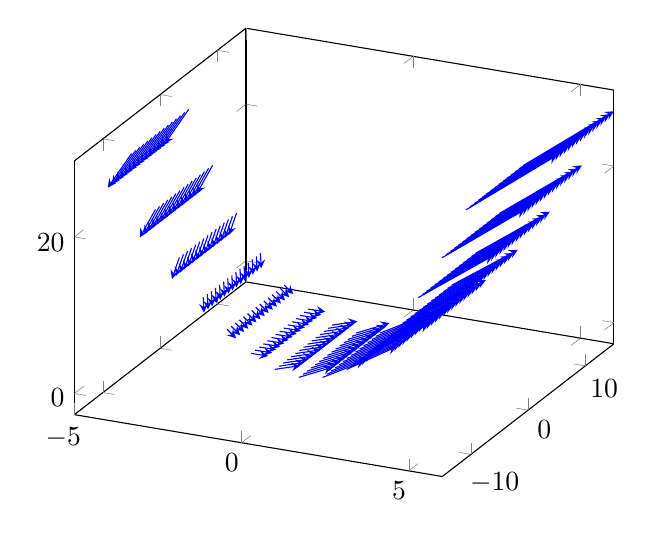
\begin{tikzpicture}
	\begin{axis}
		\addplot3[blue,
quiver={u=1,v=2*x,w=2},
-stealth,samples=15] {x^2};
	\end{axis}
\end{tikzpicture}
\end{frame}

\begin{frame}
\frametitle{Plots}
  \vspace*{-0.3cm}
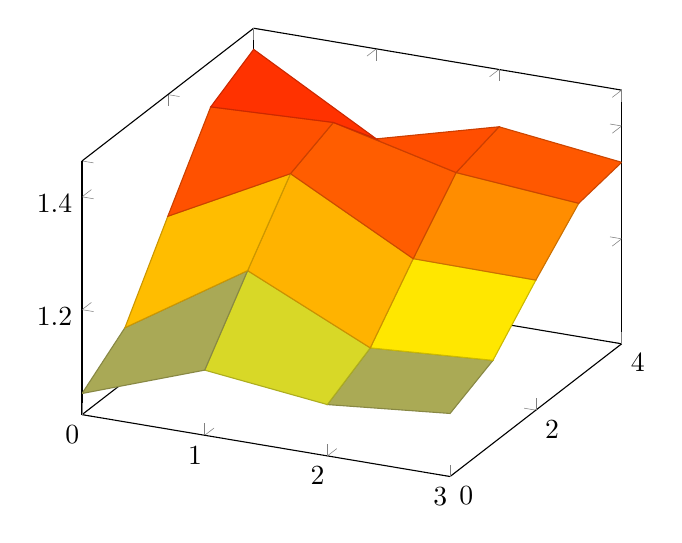
\begin{tikzpicture} 
	\begin{axis} 
\addplot3[surf] coordinates{
(0,0,1.0514) (0,1,1.1092) (0,2,1.2479) (0,3,1.3830) (0,4,1.4261)

(1,0,1.1294) (1,1,1.2470) (1,2,1.3600) (1,3,1.3920) (1,4,1.3040)

(2,0,1.1049) (2,1,1.1466) (2,2,1.2459) (2,3,1.3397) (2,4,1.3620)

(3,0,1.1257) (3,1,1.1610) (3,2,1.2445) (3,3,1.3218) (3,4,1.3356)
};
	\end{axis}
\end{tikzpicture}
\end{frame}

\begin{frame}
\frametitle{Plots}
  \vspace*{-0.3cm}
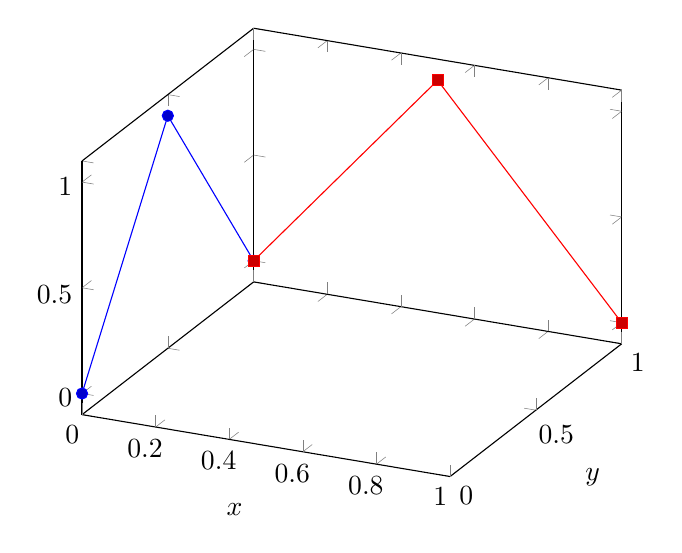
\begin{tikzpicture}
	\begin{axis}[xlabel=$x$,ylabel=$y$]
		\addplot3 coordinates {(0,0,0) (0,0.5,1) (0,1,0)};
		\addplot3 coordinates {(0,1,0) (0.5,1,1) (1,1,0)};
	\end{axis}
\end{tikzpicture}
\end{frame}

\begin{frame}
\frametitle{Plots}
  \vspace*{-0.3cm}
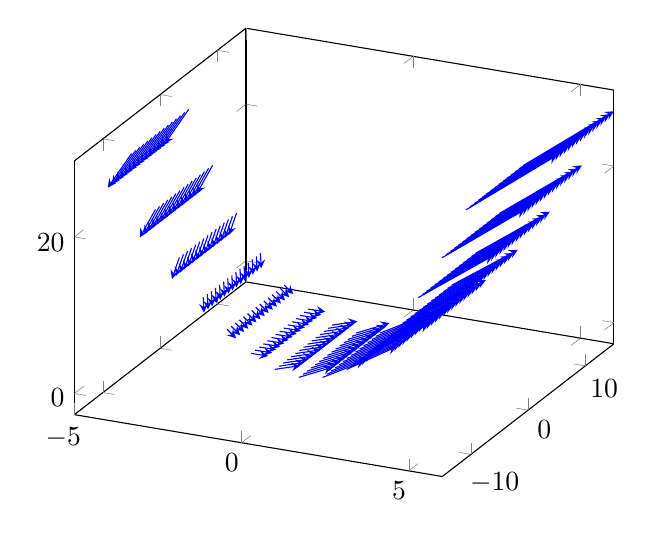
\begin{tikzpicture}
	\begin{axis}
		\addplot3[blue,
quiver={u=1,v=2*x,w=2},
-stealth,samples=15] {x^2};
	\end{axis}
\end{tikzpicture}
\end{frame}


\section{Resultate}

\subsection{Aggregatzustände} %vllt?

\begin{frame} %Beispiel, funktioniert nicht so wie ich dachte
\frametitle{Festkörper}
  \vspace*{-0.3cm}
\begin{figure}[htb]
  \centering
    \begin{tikzpicture}
      \begin{axis}[legend style={at={(0.95,0.5)},anchor=east},
          width=\linewidth,
          height=0.5\linewidth,
          xtick=data,
          xticklabels from table={dat/Potential.dat}{RANGE},
          xlabel={Range r},
          ylabel={Potential}
        ]
        \addplot table[
        x expr=\lineno,y=POTENTIAL, meta=RANGE]
        {dat/Potential.dat};

        \legend{Festkörper, Peaks bei Distanz 1,2 und 3, keine Particle näher als 1}
      \end{axis}
    \end{tikzpicture}
  %\caption{}
  \label{Plot}
\end{figure}
\end{frame}

\subsection{Noch Mögliches} %Steht erstmal irgendetwas %TODO

\begin{frame}
  \frametitle{Simulation}
    \vspace*{-0.3cm}
   \begin{block}{Einsperren}
    \begin{itemize} 
      \item Partikel in einen Block einsperren und freilassen
    \end{itemize}
  \end{block}
  \pause
  \begin{block}{Objekte}
    \begin{itemize} 
      \item unpassierbare Objekte in den Raum platzieren
      \item Semipermeable Objekte
    \end{itemize}
  \end{block}
\end{frame}

\begin{frame}
  \frametitle{Observablen}
    \vspace*{-0.3cm}
   \begin{block}{ETWAS}
    \begin{itemize} 
      \item Ein Partikel verfolgen
      \item Simulation als Gif darstellen
    \end{itemize}
  \end{block}
\end{frame}

\begin{frame}
    \vspace*{0.9cm}
    \centering
    \Huge
    Vielen Dank\\
    für\\
    Eure Aufmerksamkeit.\\
\end{frame}

\end{document}